\SECTION{Evaluation}\label{sec:evaluation}
In this section, we evaluate the runtime overhead and real-time
performance of Linux-RTXG.
The runtime overhead is classified into interrupt interception,
independent synchronization, and priority-driven scheduling in Linux.
We demonstrate that the overhead of our LKM-based real-time scheduler
for GPU applications is acceptable.
The real-time performance is verified in terms of QoS management and
prioritization using both synthetic workload and real-world
applications on top of three different device drivers -- NVIDIA,
Nouveau, and Gdev.
We demonstrate that multiple GPU applications co-scheduled by our
LKM-based real-time scheduler are successfully prioritized and
maintained at the desired frame rate even in the presence of high CPU
load.

Experiments are limited to GPU scheduling performance given that CPU
scheduling performance has already been examined in previous
work~\cite{kato2009loadable}.
Considering the results of this work and those from the previous work,
it is clarified that both emerging GPU applications and traditional CPU
applications can be managed by the real-time scheduler, without
modifying the OS kernel and device drivers.

\SUBSECTION{Evaluation Environment}
Our experiments were conducted using Linux kernel 3.16.0, an NVIDIA Geforce GTX680 GPU, a 3.40 GHz Intel Core i7 2600 (8 cores, including two hyperthreadling cores), and 8 GB main memory.
GPU programs were written in CUDA and compiled by NVCC v6.0.1.
We used the NVIDIA 331.62 driver and Nouveau Linux-3.16.0 driver.
In addition, we used NVIDIA CUDA-6.0 libraries and Gdev.

\SUBSECTION{Interrupt Intercept Overhead}
We measured the interrupt interception overhead using the Nouveau GPU driver to compare and identify the type of interrupt.
We compared elapsed time from the beginning to the end of the ISR.

\begin{figure*}[!t]
\begin{minipage}[t]{0.33\hsize}
\begin{center}
\raisebox{-3mm}{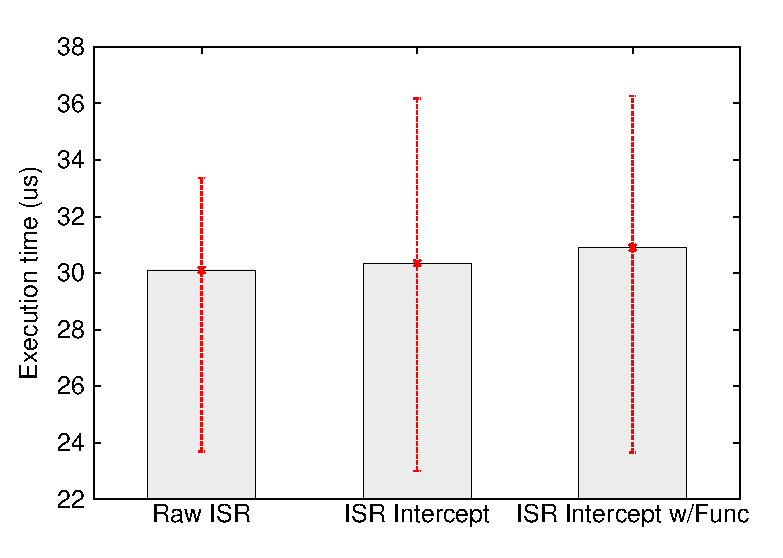
\includegraphics[width=62mm]{img/interrupt}}
\end{center}
\caption{\small{Interrupt intercept overhead \newline \,}}
\label{fig:irq_overhead}
\end{minipage}
\begin{minipage}[t]{0.33\hsize}
\begin{center}
\raisebox{-1mm}{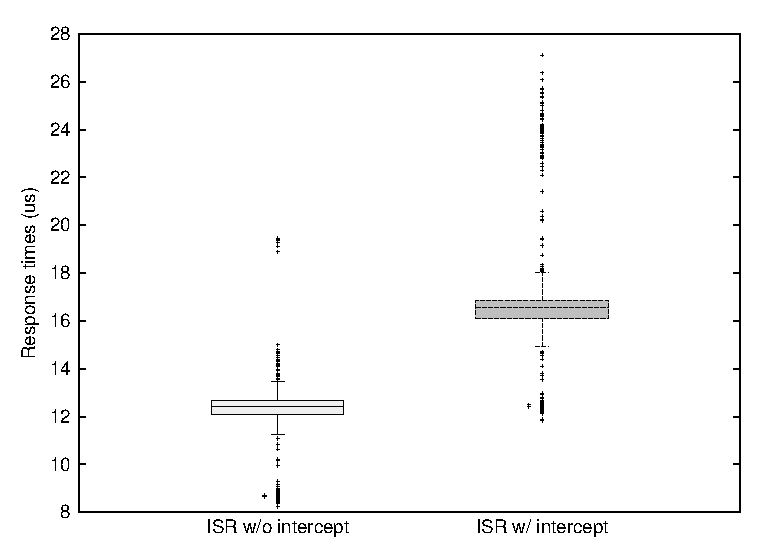
\includegraphics[width=62mm]{img/interrupt_response}}
\end{center}
\caption{\small{Response time of interrupt w/o and w/ intercept}}
\label{fig:response}
\end{minipage}
\begin{minipage}[t]{0.33\hsize}
\begin{center}
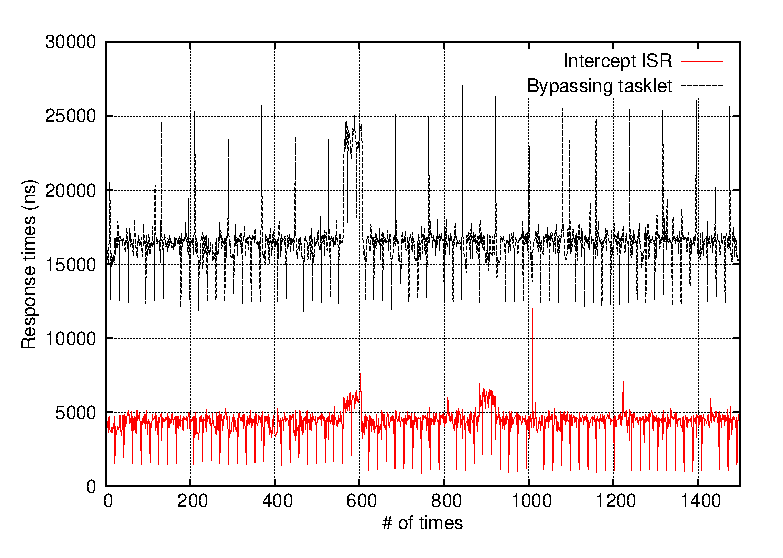
\includegraphics[width=62mm]{img/tasklet_vs_interrupt}
\end{center}
\caption{\small{Response time of the top-half intercept and bottom-half intercept}}
\label{fig:bottomvstasklet}
\end{minipage}
\end{figure*}

Figure~\ref{fig:irq_overhead} shows the results of measurements for the above setting.
Here, Raw ISR is the ISR executed in the original routine.
Note that ISR Intercept is the only intercept considered in our approach.
ISR Intercept w/Func refers to interception with processing functions that identify the ISR and wake the scheduler thread.
The results shown are average times (1000 executions); error bars indicate minimum and maximum values.

From the results, it is evident that overhead exists.
Overhead for ISR Intercept was 247 ns, which is 0.8\% of the total time required for the Raw ISR process.
Overhead for ISR Intercept w/Func was 790 ns, which is 2.6\% of the total time required for the Raw ISR process.
Intuitively, these overheads unlikely to affect the system because are very small values;
however, interrupts (e.g., timer interrupts) occur frequently, and cumulatively are likely to be significant.

Next, we compare response times to determine the impact of the interrupt intercept.
The response times are elapsed times from the start of interrupt processing to the end of identify the each interrupt type (e.g., timer, compute, FIFO, and GPIO).
The response times for ISRs with and without intercepts are shown in Figure~\ref{fig:response}.
Response times with intercepts were approximately 1.4 times longer than response times for interrupts without intercepts.
However, we target systems that do not use the GPU runtime resource management features.
Therefore, we should aim to fast response time of intercepted ISR, and original ISR response time is slow there is not affected much.

We also evaluated response time of the ISR (top-half) and the tasklet (bottom-half) in an environment to compare our results with those of previous approaches.
GPUSync intercepts the $tasklet\_schedule()$ if it is called by the NVIDIA driver.
We compare the response times of a tasklet intercept using GPUSync and the ISR intercept.
This evaluation measured response time until the responsible timing from the start of interrupt process which is $do\_IRQ$ function is called.
Figure~\ref{fig:bottomvstasklet} shows the result of this evaluation.
As can be seen, the tasklet interception response time is worse than the ISR time.
This occurs because the tasklet is typically called after significant ISR processing.

\SUBSECTION{Independent Synchronization Mechanism Overhead}
We evaluated the overhead relative to the use of an independent synchronization mechanism.
Such a mechanism must call $rtx\_nvrm\_notify()$ at the time of requested synchronization (e.g., after the kernel launch request) and $rtx\_nvrm\_init()$.
In vanilla environments, Linux-RTX's APIs are not necessary.
Therefore, overhead includes the API execution time.
We measured overhead by measuring API execution time between each API call and return.

\begin{figure}[!t]
\begin{center}
\subfigure[Part of Initialize]{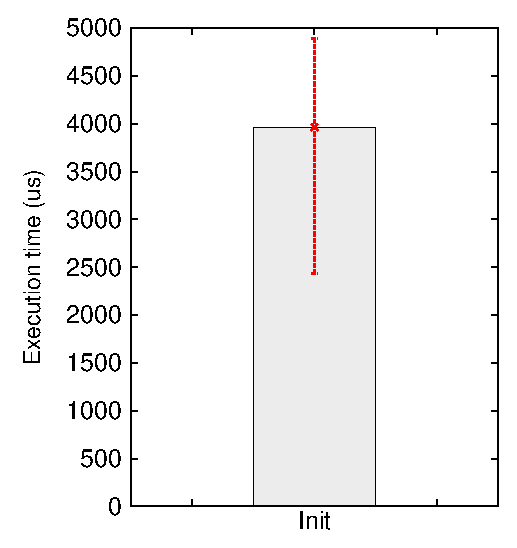
\includegraphics[width=0.23\textwidth]{img/irq_rise_init.eps}}\subfigure[Part of notify]{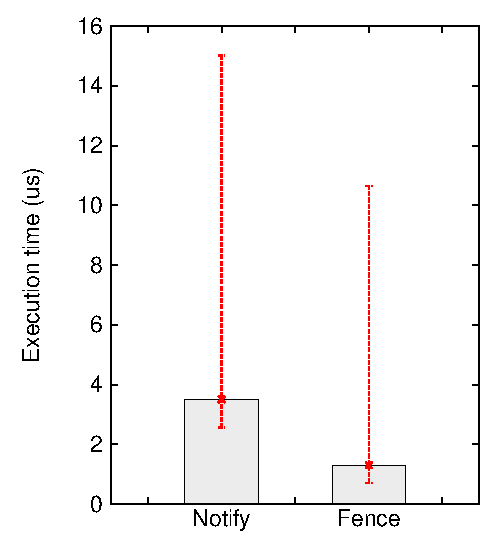
\includegraphics[width=0.22\textwidth]{img/irq_rise_notify.eps}}
\caption{Interrupt raised method overhead}
\label{fig:irq_rise_overhead}
\end{center}
\end{figure}

Figure~\ref{fig:irq_rise_overhead} shows the measurement results.
Initilize part is required to call a Linux process to allocate an indirect buffer and registers several engines such as compute and copy to the device driver.
Notification ($rtx\_gpu\_notify()$) insert commands into a command steram to GPU devices that are called when synchronization is required, such as after a kernel launch is issued.
Execution time have scatters that are affected by an ioctl system call.
The average Initizalize time is approximately 4 millseconds.
However, applications are not affected significantly because Initialize is only called once.
Notification's NOTIFY requires approximately 3.5 microseconds and FENCE requires approximately 2 microseconds.
Consequently, the time required by these method is not a major consideration for applications.
However, overhead must be considered in a shot application cycle.

\SUBSECTION{Scheduling Overhead}\label{sec:eval:sched_overhead}

\begin{figure}[!t]
\begin{center}
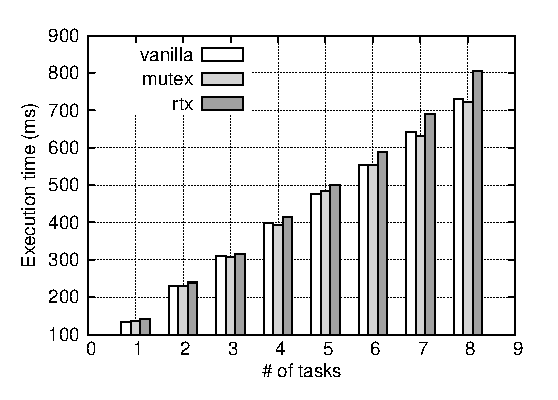
\includegraphics[width=.44\textwidth]{img/sum_task.eps}
\caption{Scheduling overhead (Time of entire task)}
\label{fig:fp_task_overhead}
\end{center}
\end{figure}

We evaluated scheduling overhead using the proposed Linux-RTXG scheduler.
We prepared three applications, i.e., vanilla, mutex, and rtx to measure overhead.
These applications are based on a common application that is Gdev's microbenchmark, which has a GPU looping function.
%details
Changes were arranged to generate multiple GPU tasks by the $fork()$ systemcall.
Each task has 10 jobs, and each job includes GPU data transfer and GPU kernel execution.
The rtx application was scheduled by rtx.
The mutex application was limited to a single kernel issue by exclusion control using mutex similar to rtx.
The vanilla application was not changed.
The CPU scheduling policy used in this evaluation was the simple fixed-priority scheduling of the proposed Linux-RTXG, which is similar to Linux's $SCHED\_FIFO$. Note that the difference between these policies is the presence or absence of job management.
The GPU scheduling policy is the fixed-priority scheduling with resource reservation, i.e., BAND scheduling policy.
Here, synchronization is used NOTIFY of the independent synchronization mechanism.

We measured the average time in 100 times GPU task execution (1000 jobs).
The result shows in Figure~\ref{fig:fp_task_overhead}.
Overhead increases in proportion as the number of tasks increases because task scheduling processing times is increased.
Max overhead is 10\% at the eight tasks based on "vanilla" time.

\SUBSECTION{Performance of QoS management}
Experiments were also performed to evaluate QoS management performance.
In this evaluation, we measured the utilization of each tasks in several environments,
which indicates whether performance is affected by kernel modification.

\begin{figure*}[!t]
\begin{minipage}[t]{0.33\hsize}
\begin{center}
\subfigure[{\small FIFO with NVIDIA}]{
\includegraphics[width=62mm]{img/fifo_rtx_nvidia}} 
\label{fig:fifo_rtx_nvidia} \\
\subfigure[{\small BAND with NVIDIA}]{
\includegraphics[width=62mm]{img/band_rtx_nvidia}}
\label{fig:band_rtx_nvidia}
\label{fig:rtx_nvidia}
\end{center}
\end{minipage}
\begin{minipage}[t]{0.33\hsize}
\begin{center}
\subfigure[{\small FIFO with Nouveau}]{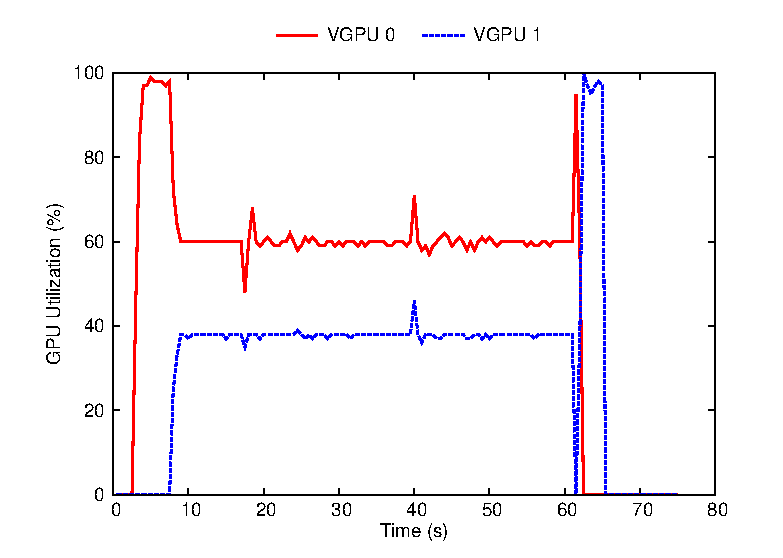
\includegraphics[width=62mm]{img/fifo_rtx}}
\label{fig:fifo_rtx} \\
\subfigure[{\small BAND with Nouveau}]{
\includegraphics[width=62mm]{img/band_rtx}}
\label{fig:band_rtx}
\label{fig:rtx_nouveau}
\end{center}
\end{minipage}
\begin{minipage}[t]{0.33\hsize}
\begin{center}
\subfigure[{\small FIFO on Gdev}]{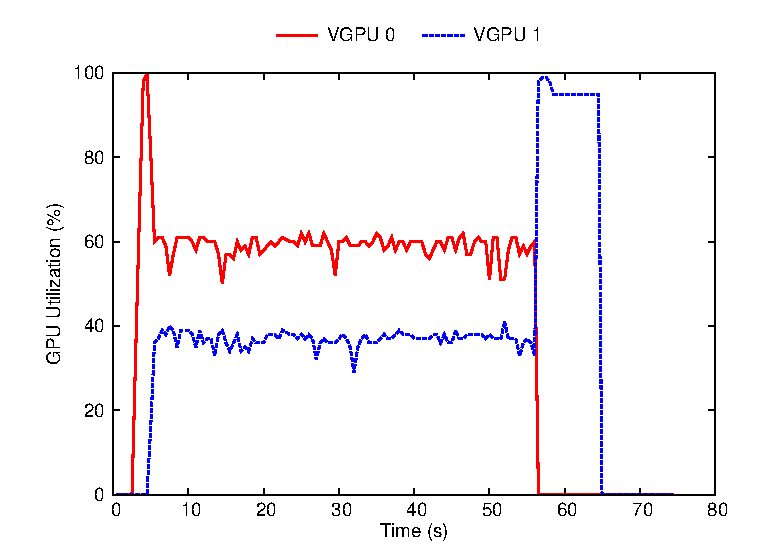
\includegraphics[width=62mm]{img/fifo_gdev}}
\label{fig:fifo_gdev} \\
\subfigure[{\small BAND on Gdev}]{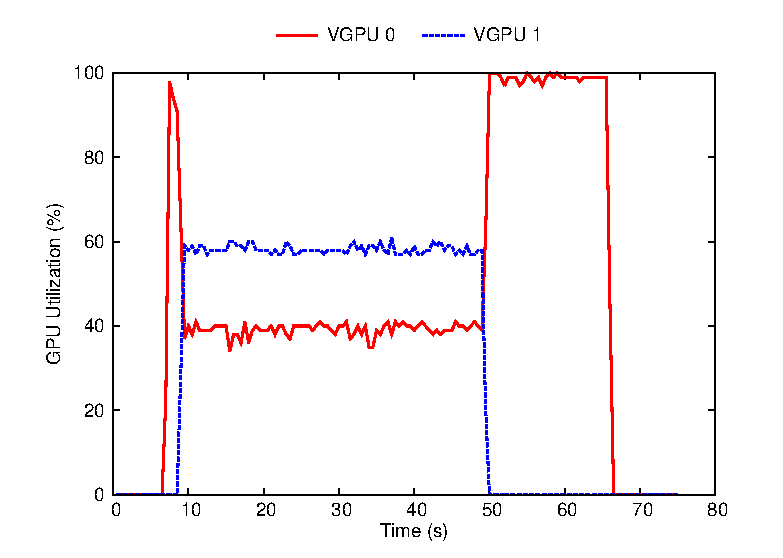
\includegraphics[width=62mm]{img/band_gdev}}
\label{fig:band_gdev}
\label{fig:gdev_usage}
\end{center}
\end{minipage}
\caption{Utilization of two tasks with each scheduler. Each task had different workloads and different resource allocations (VGPU0 = 40\%, VGPU1 = 60\%).}
\label{fig:utilize}
\end{figure*}

\begin{figure}[!t]
\begin{center}

\includegraphics[width=0.4\textwidth]{img/band_rtx_fair}
\caption{Utilization of four tasks with the Linux-RTXG's BAND VGPU scheduling. Each tasks had a equal workload and a equal GPU resource allocation.}
\label{fig:band_rtx_fair}
\end{center}
\end{figure}

QoS performance use an indication of whether the task of the resource is guaranteed.
We evaluate task isolation performances with Linux-RTXG's GPU scheduler using the NVIDIA GPU driver and the Nouveau GPU driver to confirm the guaranteed resources.
First, we measured the utilization when running two GPU tasks.
Each GPU tasks had a different workload and a different GPU resource.
One GPU task was allocated VGPU0, and given the 40\% GPU resource.
This task has about 1.2 times the workload of other tasks.
The other GPU task was allocated VGPU1 and given the 60\% GPU resource.
VGPU1 task was scheduled to start approximately 5 safter the VGPU0 task.

Figure~\ref{fig:utilize}(a) shows result of FIFO scheduling policies on the NVIDIA Driver,
and the BAND scheduling policies is shown in Figure~\ref{fig:utilize}(b).

The Nouveau GPU driver results are shown in Figures~\ref{fig:utilize}(c) and (d).
The FIFO scheduling policies shown in Figure~\ref{fig:utilize}(c),
and the BAND scheduling policies shown in Figure~\ref{fig:utilize}(d).

The results shown in Figure~\ref{fig:utilize}(a) and (c) indicate that the GPU tasks are performed in accordance with the workload by fair scheduling.
The results shown in Figure~\ref{fig:utilize}(b) and \ref{fig:utilize}(d) indicate that the GPU tasks are performed in accordance with the utilization by resource reservation mechanisms.

The VGPU1 task's maximum error was approximately 3\% for the initial BAND scheduling policies' resource management using the NVIDIA GPU driver.
The VGPU0 task's maximum error was approximately 5\%.
The VGPU1 task's maximum error was approximately 2\% under the initial BAND scheduling policies' resource management using the Nouveau GPU driver.
The VGPU0 task's maximum error was approximately 2\%.
Large spikes occurred due to GPU kernel overrun.
If the GPU scheduler need to large spike is reduced, the GPU scheduler is needed for runtime approaches such as making preemptive GPU kernel.

In addition, we compare performance with prior work that is Gdev.
The Gdev scheduling results are shown in Figures~\ref{fig:utilize}(e) and (f).
Linux-RTXG is seen almost no performance degradation as compared with Gdev.
In details, the VGPU1 task's maximum error was approximately 3\% for the initial BAND scheduling policies' resource management using the Gdev scheduler.
The VGPU0 task's maximum error was approximately 5\%.
We guess that there is a large variation caused by runtime specification of the Gdev function must through the kernel module using Gdev scheduler.

We then measured utilization running four GPU tasks.
Each GPU tasks had equal workload and equal GPU resource allocation.
In addition, each GPU task was allocated to each VGPU.
Results for BAND scheduling policies are shown in Figure~\ref{fig:band_rtx_fair}.
A maximum error of these VGPUs was appropriately 9\%, it values are occurred because of the timing of budget replenishment and a synchronization latency.  

Therefore, the results show that the synchronization mechanism of the proposed Linux-RTXG can schedule tasks without sacrificing performance.

\begin{figure*}[!t]
\begin{minipage}[t]{0.33\hsize}
\begin{center}
\subfigure[{\small NULL}]{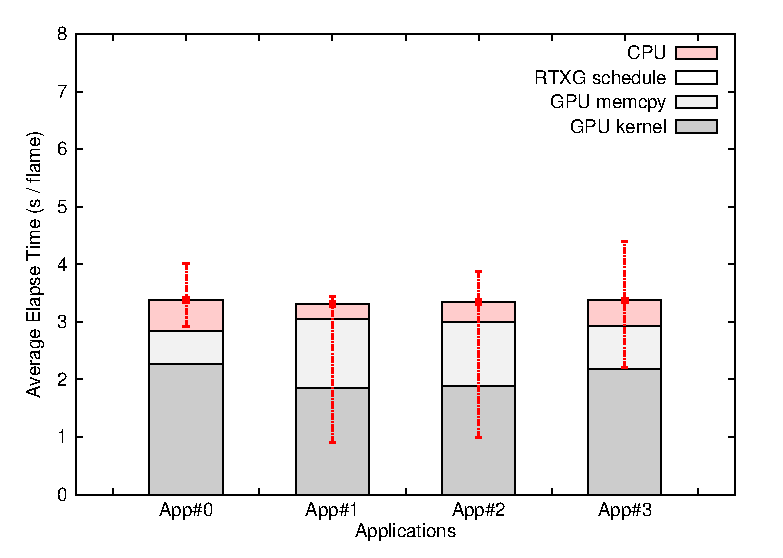
\includegraphics[width=62mm]{img/real_null_null_withoutload}}
\label{fig:real-null_null}
\subfigure[{\small FP}]{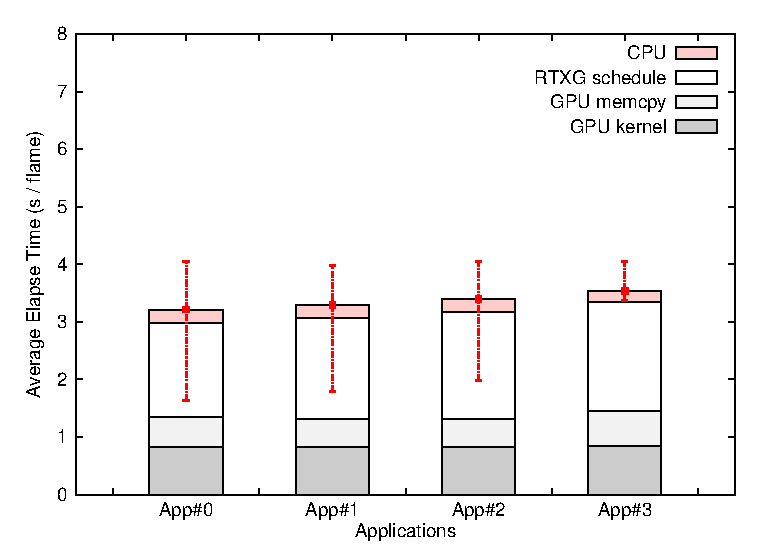
\includegraphics[width=62mm]{img/real_prio_null_withoutload}}
\label{fig:real-prio_null}
\end{center}
\end{minipage}
\begin{minipage}[t]{0.33\hsize}
\begin{center}
\subfigure[{\small BAND}]{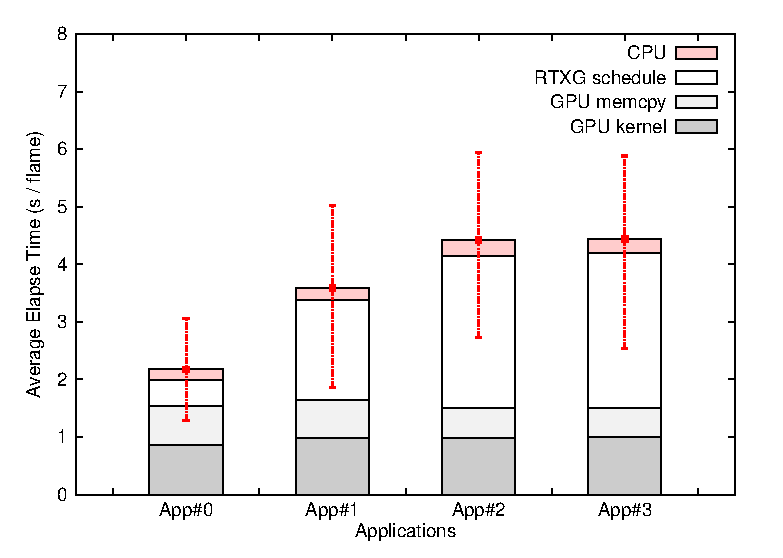
\includegraphics[width=62mm]{img/real_prio_band_withoutload}}
\label{fig:real-prio_band}
\subfigure[{\small BAND with high CPU load}]{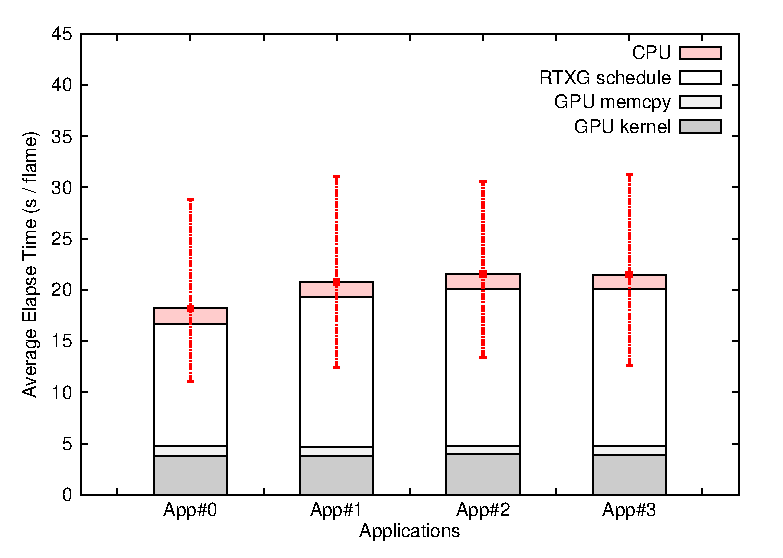
\includegraphics[width=62mm]{img/real_prio_band_withhighload}}
\label{fig:real-prio_band-hiload}
\end{center}
\end{minipage}
\begin{minipage}[t]{0.33\hsize}
\begin{center}
\subfigure[{\small NULL with high CPU load}]{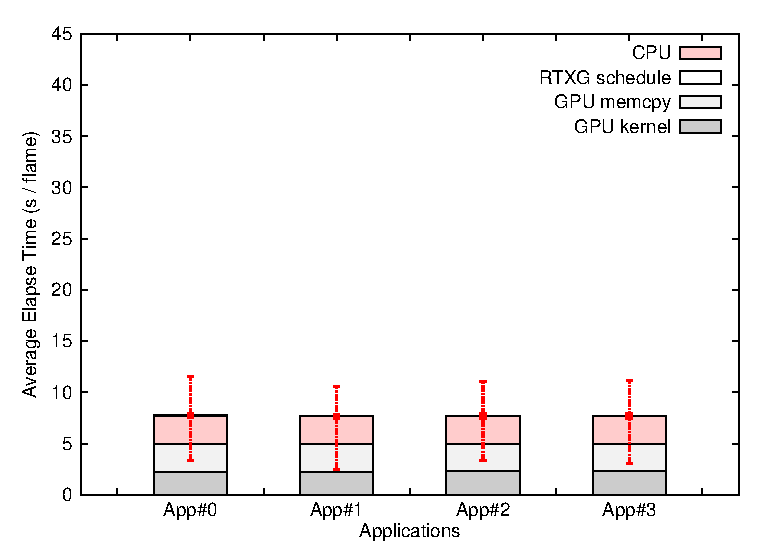
\includegraphics[width=62mm]{img/real_null_null_withhiload}}
\label{fig:real-null_null-hiload}
\subfigure[{\small G-RM and BAND with high CPU load}]{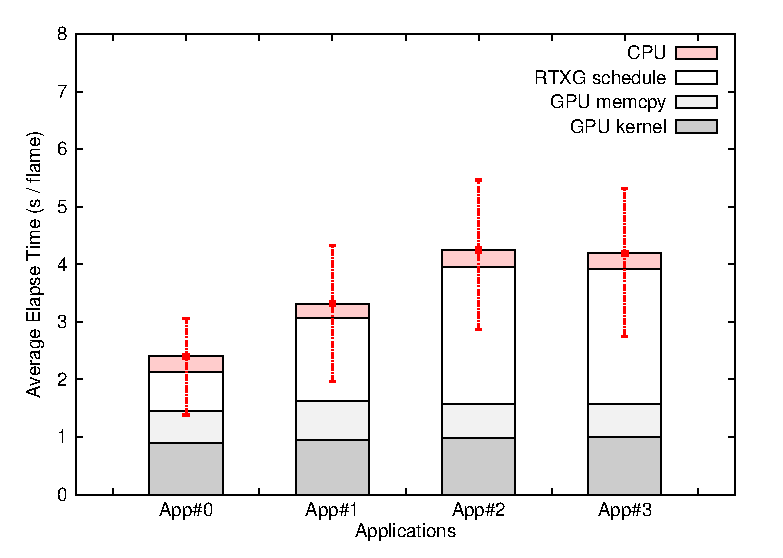
\includegraphics[width=62mm]{img/real_prio_band_withhighload_cpu}}
\label{fig:real-prio_band_cpu-hiload}
\end{center}
\end{minipage}
\caption{Elapse times of object detection applications on various situation.}
\label{fig:elapse_time_all}
\end{figure*}

\SUBSECTION{Real-world Application}
Here, we demonstrate scheduling performance using real-world oriented application.
We employed real-world oriented application which is object detection application using the HOG features.
We run four tasks are assumed to recognize the four directions that are forward, backward, right, and left.

Algorithms and implementation of the applications are described in the previous work~\cite{hirabayashi:cpsna2013}.

We measure the elapse time of processing one frame image in six situations.
Each situation results are shown in Figure~\ref{fig:elapse_time_all}.
Each GPU tasks are allocated difference resources are given 60\%, 20\%, 10\%, and 10\% respectively.
Figure~\ref{fig:elapse_time_all}(a) is shown result of executing four tasks without scheduling.
All tasks are performed equally on its situation.
Figure~\ref{fig:elapse_time_all}(b) is shown result on executing four task runnning with a fixed-priority GPU kernel scheduling (FP).
If a scheduler only uses fixed-priority GPU kernel scheduling, tasks are almost the same as the Figure~\ref{fig:elapse_time_all}(a).
Figure~\ref{fig:elapse_time_all}(c) is addition of the BAND VGPU scheduling from the Figure~\ref{fig:elapse_time_all}(b) situation.
In this case, the tasks have been adapted the priority of each tasks for which can suppress the GPU kernel execution.
Figures~\ref{fig:elapse_time_all}(d) and (e) are shown result of the high CPU load environment.
Note that high CPU load is generated by hackbench tasks as known as an UNIX's standard stress test tool.
High CPU load tasks policy is Linux's $SCHED\_OTHER$.
If an OS has some high-CPU load tasks, GPU tasks do not work well using only GPU scheduling
because GPU tasks can not acquire the CPU to issue an API due to other tasks.
Such a high-CPU load environment to occur well in autonomouse driving car systems because the systems require a lot of applications (e.g., SLAM, Navigation, and Car control) despite limit the resources.
Linux-RTXG can provide real-time CPU scheduling and GPU scheduling.
Therefore, Linux-RTXG can solves problem due to other CPU tasks.
The result show in Figure~\ref{fig:elapse_time_all}(f).
As can be seen, applications are not affected high-CPU load task by fixed-priority CPU scheduling (G-RM:Glocbal Rate-monotonic).
These experimental results indicate that Linux-RTX making the adequate performance for real-world oriented applications.

